\documentclass{article}

\title{Práctica 3 de Criptografía y Computación}
\date{}
\author{Carlos Núñez Molina \\ Alessandro Zito \\ Gabriela Antolinez}

\usepackage{titlesec}
\usepackage{graphicx}



\titleformat{\section}
  {\normalfont\large}{\thesection}{}

\begin{document}
	\maketitle
	\newpage

    \section{Análisis de tiempos para Factorización}

    En esta sección vamos a analizar cuánto se tarda en factorizar varios números. Para ello utilizaremos tres algoritmos diferentes: Fuerza Bruta, Fermat y Ro de Pollard. Hemos hecho los análisis de frecuencias con números al azar y con números productos de primos. Hemos factorizado los números completamente (no encontramos un solo factor sino todos los factores), y se fue analizando cómo varía la eficiencia de los algoritmos según aumenta el número de cifras (en formato decimal, no binario). Además, hemos hecho experimentos para dos tipos de números: aquellos elegidos al azar y aquellos que son producto de dos primos de forma que el número resultante tiene n cifras.
    
Ahora se presenta el análisis de los algoritmos con los números elegidos al azar.

    \subsection{Fuerza Bruta}
    Empezando con el algoritmo de Fuerza Bruta, sabemos que este algoritmo va probando números de manera ascendente para ver si alguno es divisor. Podemos ver en la primera imagen que el algoritmo es capaz de factorizar números de hasta 28 cifras, a partir de los cuales ya tarda demasiado. Su eficiencia es exponencial en el número de cifras, llegando a tardar \begin{math} 10^{2} \end{math} segundos cuando el número tiene 28 cifras.



    \begin{figure}[ht!]
        \centering
        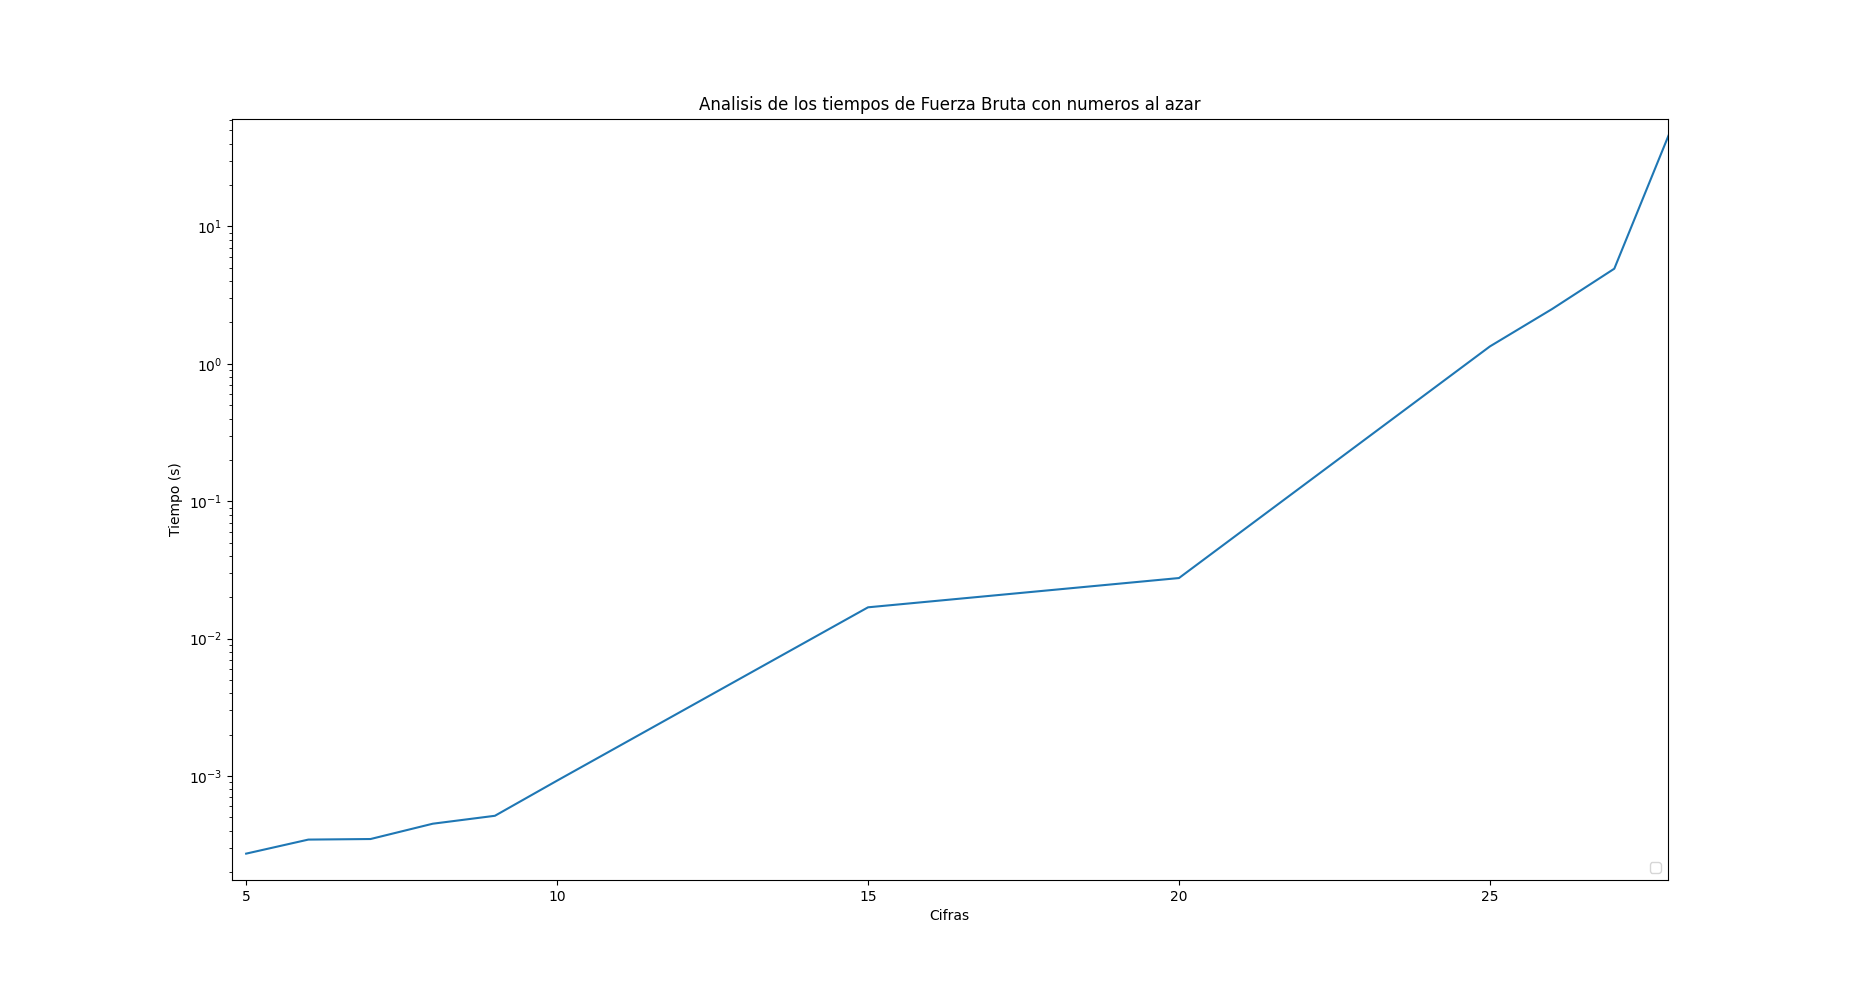
\includegraphics[width=\linewidth]{Figure_1}
        \caption{Análisis de los tiempos de Fuerza Bruta con números al azar}
        \label{fig:Figure_1}
    \end{figure}

    \newpage

    \subsection{Fermat}
    Siguiendo con el algoritmo de Fermat, sabemos que este algoritmo va a resolver la ecuación \begin{math} y = x ^{2} - n \end{math} para factorizar el número. Se puede observar en la imagen que este algoritmo es el peor de los tres, ya que sólo es capaz de factorizar en un tiempo razonable números de hasta 10 cifras. El algoritmo es el peor de los tres por cómo realiza la factorización de los números dado que utiliza la forma \begin{math} (x-n)*(x+n)\end{math}. Así, estos dos factores tienen que estar próximos entre sí (y de la raíz cuadrada del número a factorizar) para que el método funcione bien (si no lo están, tarda mucho). Por eso con los números elegidos al azar es tan ineficiente, ya que suelen tener divisores pequeños.



    \begin{figure}[ht!]
        \centering
        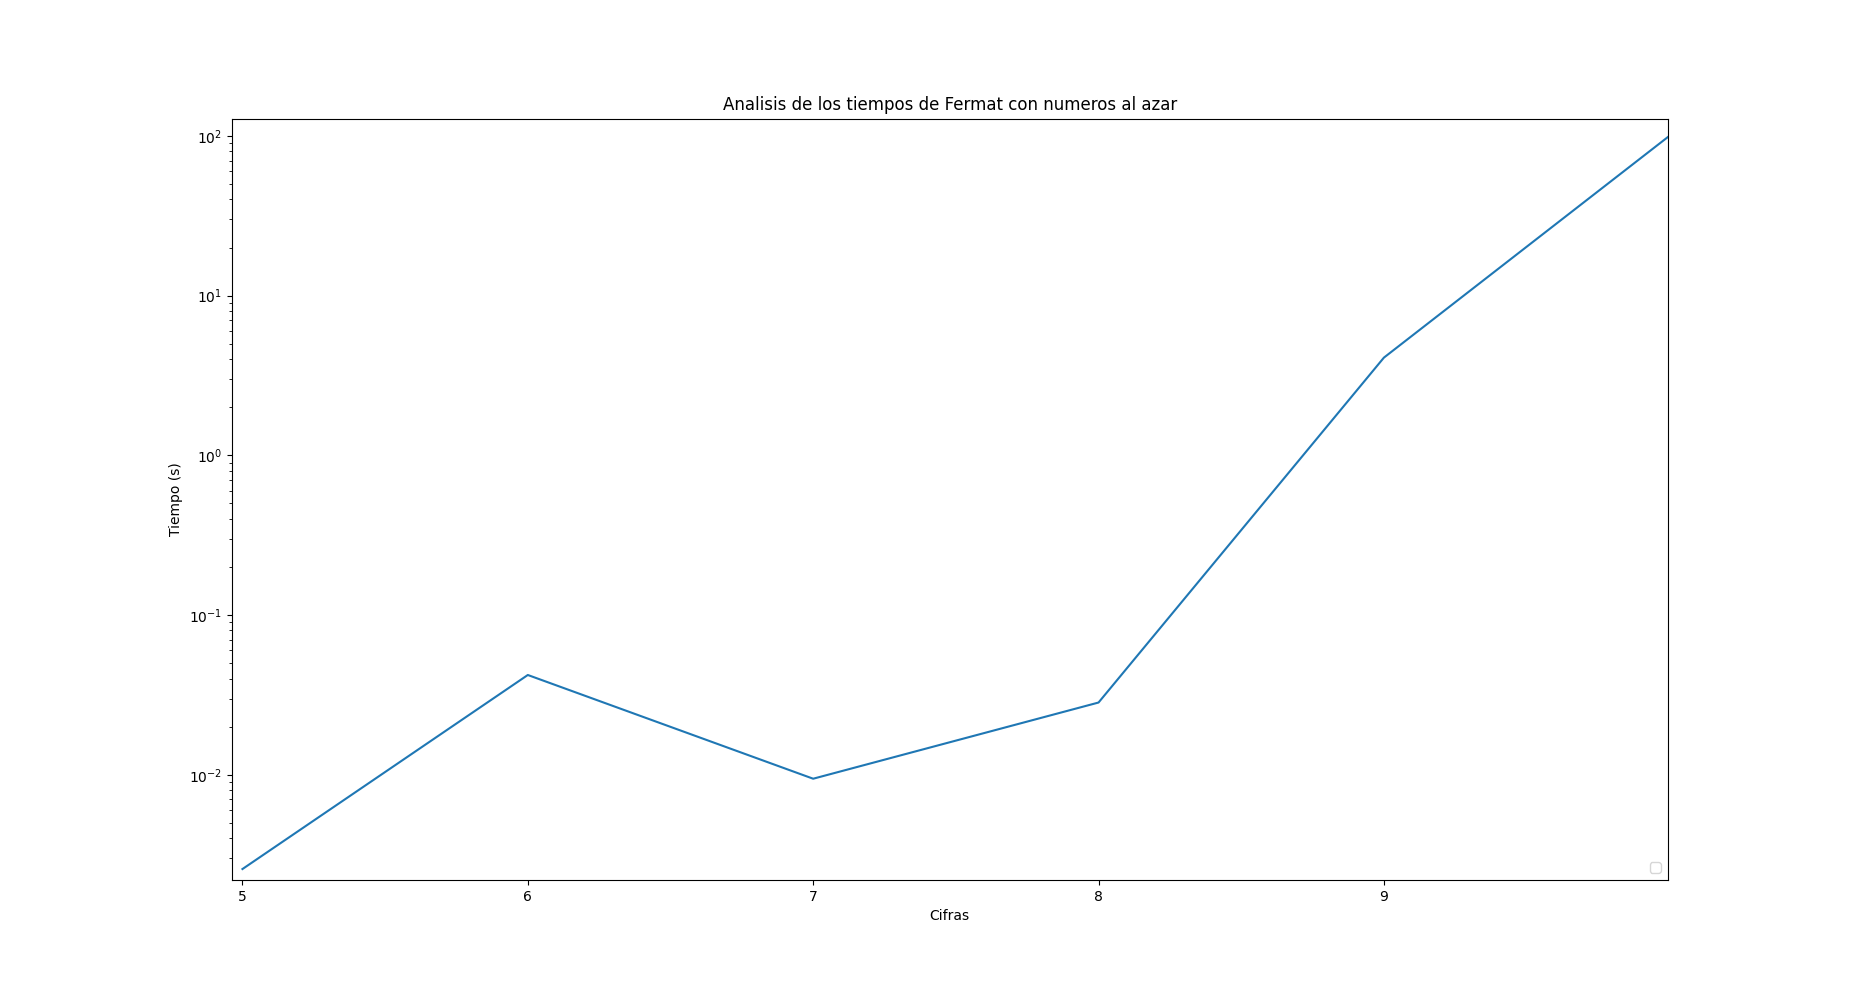
\includegraphics[width=\linewidth]{Figure_3}
        \caption{Análisis de los tiempos de Fermat con números al azar}
        \label{fig:Figure_3}
    \end{figure}

    \newpage

    \subsection{Ro de Pollard}
    El último de los tres métodos estudiados es el algoritmo Ro de Pollard, que tiene el nombre del matemático que lo inventó. Se trata de construir una sucesión
    \begin{math} x_{1}, x_{2}, ..., x_{n} \end{math} y encontrar dos términos de la sucesión
    \begin{math}  x_{i}, x_{j} \end{math} tales que \begin{math} mcd(x_{i} - x_{j} ; n) \neq 1. \end{math} Podemos ver que este algoritmo es el más eficiente de los 3 estudiados dado que tarda solo 100 segundos para factorizar números de 42 cifras.


    \begin{figure}[ht!]
        \centering
        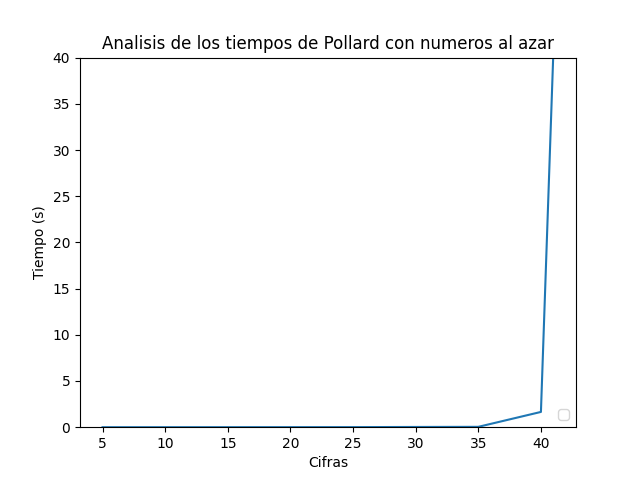
\includegraphics[width=\linewidth]{Figure_5}
        \caption{Análisis de los tiempos de Pollard con números al azar}
        \label{fig:Figure_5}
    \end{figure}


    \newpage


    Haciendo los mismos test pero ahora con números productos de dos primos, se puede ver cómo los algoritmos siguen siendo exponenciales en el número de cifras. Además, se ve cómo Fuerza Bruta y Pollard tardan más porque los números son más difíciles de factorizar: tienen solo dos factores y son más grandes que cuando los números se eligen al azar. Sin embargo, Fermat tarda menos con este tipo de números porque ambos factores están más cerca entre sí y de la raíz cuadrada del número. 
    El mejor algoritmo sigue siendo Pollard dado que factoriza hasta 28 cifras, sin embargo los rendimientos de Fuerza Bruta y Fermat se han vuelto más equiparables, aunque Fuerza Bruta sigue siendo mejor que Fermat dado que llega a factorizar 20 cifras y Fermat sólo 18 cifras.

    \begin{figure}[ht!]
        \centering
        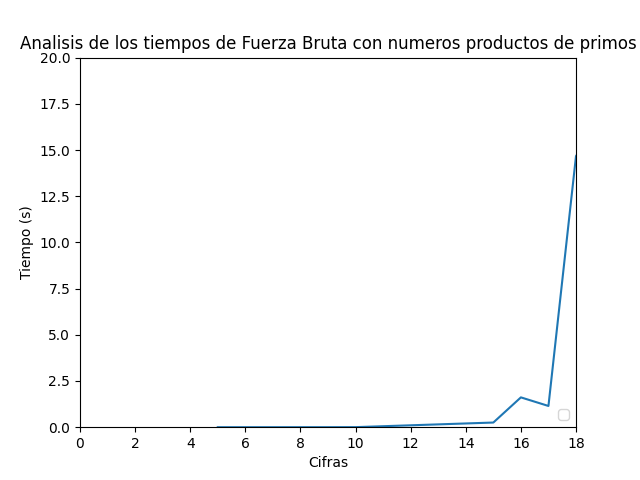
\includegraphics[width=\linewidth]{Figure_2}
        \caption{Análisis de los tiempos de Fuerza Bruta con números productos de dos primos}
        \label{fig:Figure_2}
    \end{figure}

    \begin{figure}[ht!]
        \centering
        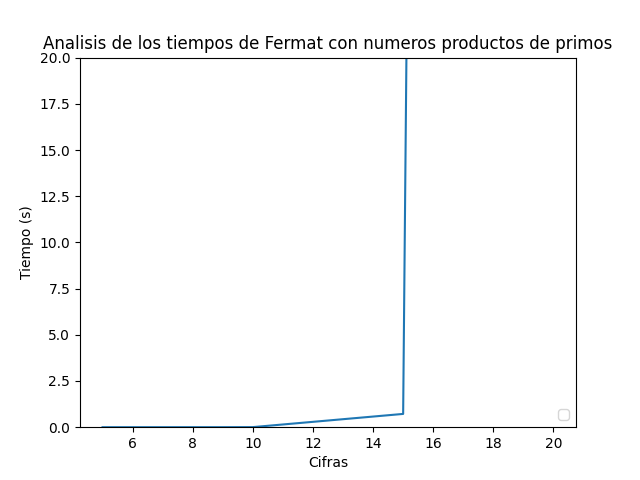
\includegraphics[width=\linewidth]{Figure_4}
        \caption{Análisis de los tiempos de Fermat con números productos de dos primos}
        \label{fig:Figure_4}
    \end{figure}

    \begin{figure}[ht!]
        \centering
        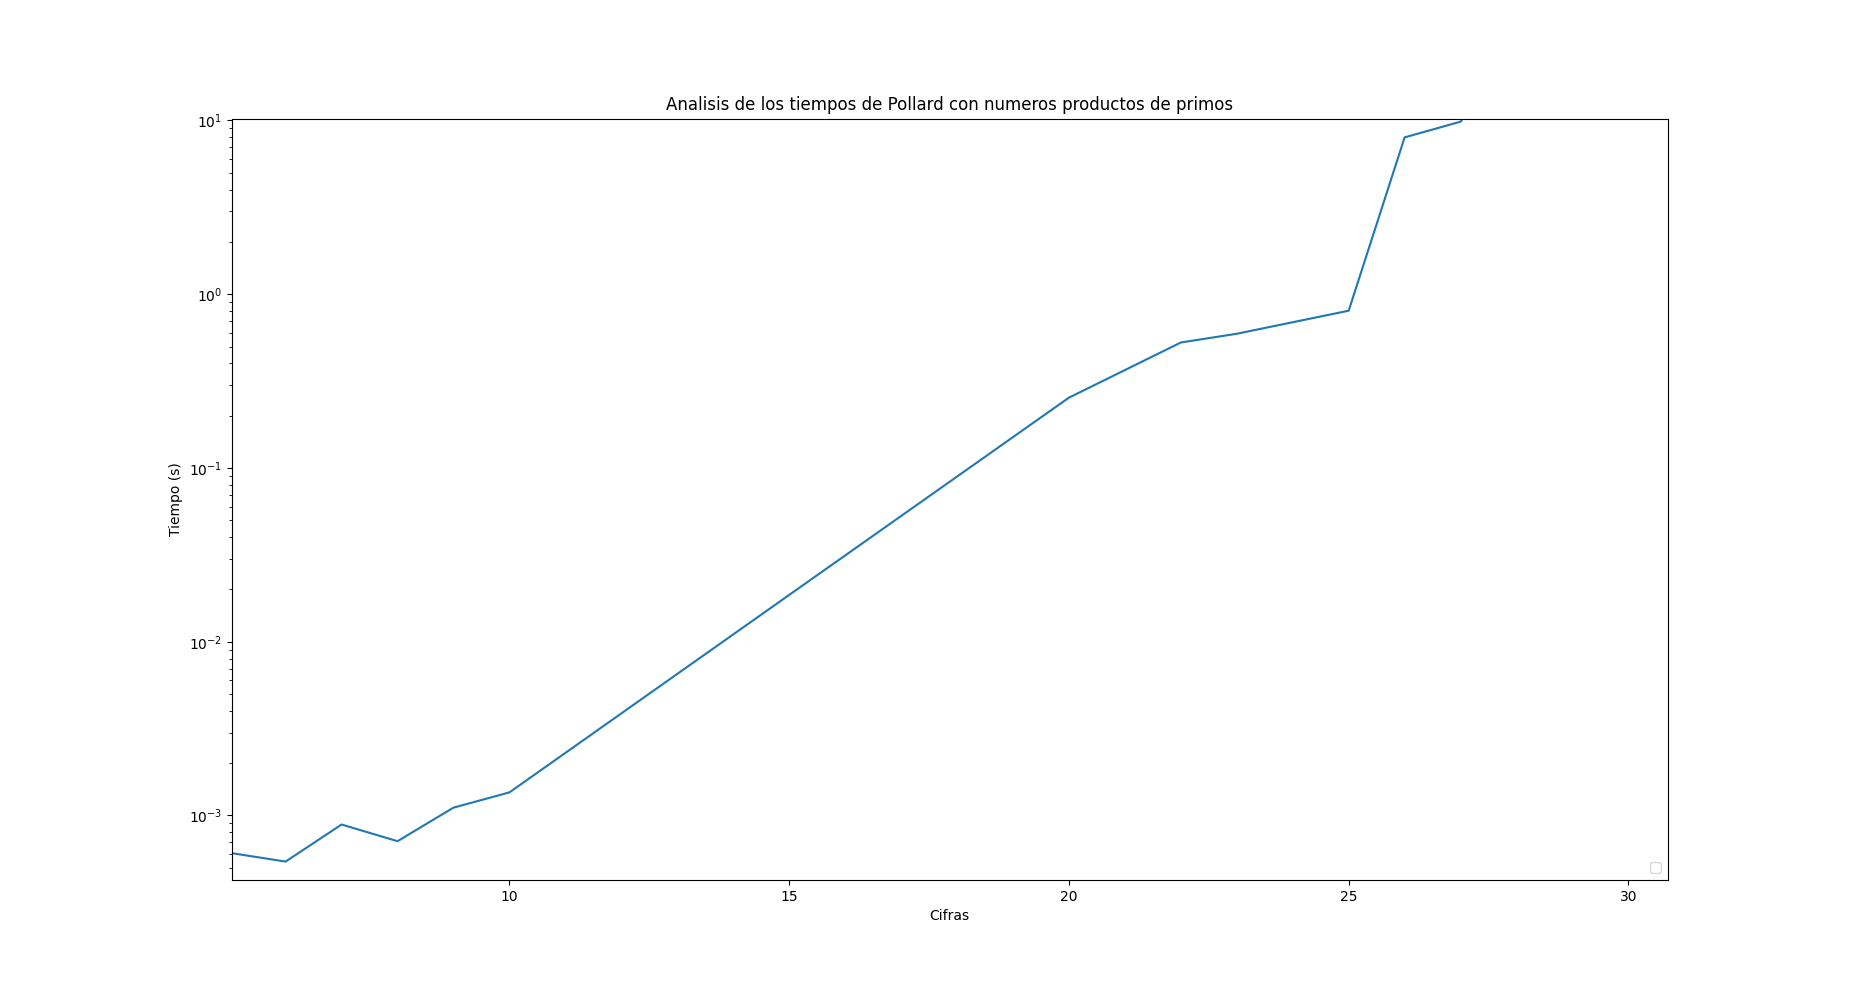
\includegraphics[width=\linewidth]{Figure_6}
        \caption{Análisis de los tiempos de Pollard con números productos de dos primos}
        \label{fig:Figure_6}
    \end{figure}
 \newpage
 
\subsection*{Estimaciones}
    Hemos hecho una  estimación para ver cuánto tarda cada algoritmo con un número de 50 cifras. La estimación se ha realizado de la siguiente forma: se ha calculado para cada algoritmo cuánto tarda más de media en factorizar un número con una cifra más. Para calcular esta media, no se han tenido en cuenta los tiempos pequeños, ya que son muy imprecisos. Una vez calculada, se ha usado para estimar el tiempo medio de cada algoritmo para un número de 50 cifras. Los resultados se detallan a continuación:
    
    \begin{itemize}
        \item Fuerza Bruta:
        \begin{itemize}
            \item Número de 50 cifras al azar: 1.394766457605177e+34
            \item Número de 50 cifras producto de primos: 2.1029773066486474e+80
        \end{itemize}
        \item Fermat:
        \begin{itemize}
            \item Número de 50 cifras al azar: 2.2167256626584056e+68
            \item Número de 50 cifras producto de primos: 4.378776394397684e+74
        \end{itemize}
        \item Ro de Pollard:
        \begin{itemize}
            \item Número de 50 cifras al azar: 5.995733542705329e+30
            \item Número de 50 cifras producto de primos: 2.9305515186779655e+20
        \end{itemize}
    \end{itemize}

    \subsection*{Conclusiones de análisis de tiempos para Factorización}
    A partir de estos resultados evidenciamos que ninguno de los algoritmos es capaz de factorizar números de 50 cifras (incluso el mejor de ellos tardaría billones de años). Como se puede ver, Pollard tarda menos en calcular el número en ambas formas. Fermat tarda menos que Fuerza Bruta en números producto de primos pero sigue siendo el peor de los tres. Por tanto, consideramos que el peor de los tres métodos es Fermat: funciona peor que Fuerza Bruta para números al azar y cuando son producto de primos funciona mejor pero sigue siendo peor que fuerza bruta. El mejor de los tres métodos es Pollard, ya que es el mejor sin importar si los números son escogidos al azar o producto de primos.


    \newpage
    \section{Análisis de tiempos para Logaritmo discreto}
    Al igual que en la sección anterior se realiza un análisis de tiempos, en este caso, para hallar la solución del logaritmo discreto. Para ello se estudian tres algoritmos: Fuerza Bruta, Paso Enano - Paso Gigante y Ro de Pollard. 
    Con el fin de conocer la eficiencia de los algoritmos, se realiza la evaluación con los mismos números para cada uno de los tres algoritmos, cuyas cifras irán aumentando para estudiar cuánto tiempo tarda en llegar a la solución del logaritmo.
    
    \subsection{Fuerza Bruta}
    Este algoritmo realiza la evaluación de las distintas potencias de \begin{math}a^i\end{math} siendo i un número entre \begin{math} 0\leq i \leq p-2 \end{math} hasta que la potencia encontrada sea \begin{math}b\end{math}. Así, el algoritmo logra encontrar la solución del logaritmo. Sin embargo, presenta problemas respecto a su eficiencia dado que aumenta de manera desmesurada el tiempo para encontrar la solución conforme se aumenta el número de cifras. Esto es debido a que el algoritmo debe evaluar un número de potencias equivalente al tamaño de $p$.
     \begin{figure}[ht!]
        \centering
        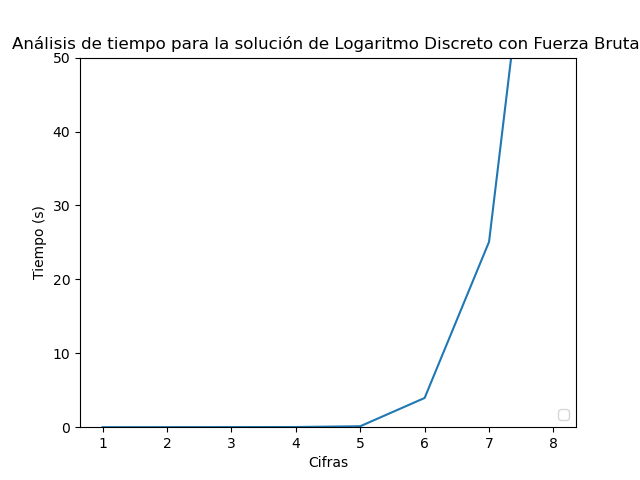
\includegraphics[width=\linewidth]{Figure_7}
        \caption{Análisis de los tiempos de Fuerza Bruta para PLD.}
        \label{fig:Figure_6}
    \end{figure}
    \newpage
    
    \subsection{Paso Enano - Paso Gigante}
    En este algoritmo la solución es escrita como \begin{math}x=t*s-i\end{math}, la cual es resultado de realizar la comparación entre los números \begin{math}S={b,b*a,b*a^2,...,b*a^{s-1}}\end{math} y \begin{math}{a^s,a^{s*2},...,a^{s^2}}\end{math}. El comportamiento de este método comienza a deteriorarse conforme se va aumentando el número de cifras existentes,lo que provoca que el número de comparaciones entre los dos conjunto de números resulte excesivo, dado que cada elemento de \begin{math}{a^s,a^{s*2},...,a^{s^2}}\end{math} debe compararse \begin{math}{s}\end{math} veces.
    \newblock
    Así, si el número primo p tiene gran cantidad de cifras, su raíz \begin{math}{s}\end{math} será grande de igual forma, por lo que el número de comparaciones a realizar es muy grande.
     \begin{figure}[ht!]
        \centering
        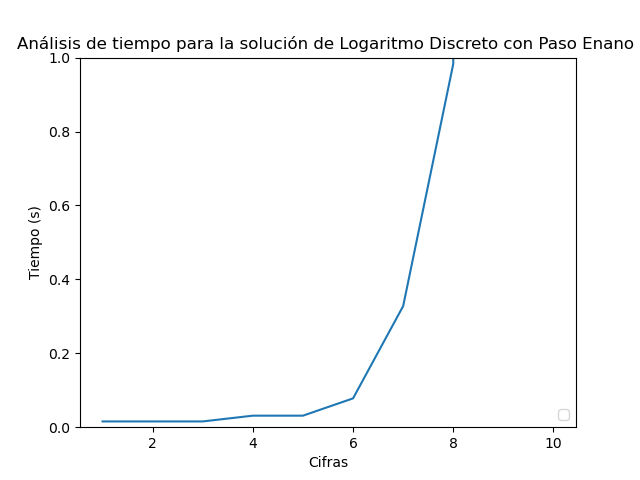
\includegraphics[width=\linewidth]{Figure_8}
        \caption{Análisis de los tiempos de Paso Enano - Paso Gigante para PLD.}
        \label{fig:Figure_6}
    \end{figure}
    \newpage
    
    \subsection{Ro de Pollard}
    Por último, el algoritmo de Pollard consiste en la generación de una sucesión pseudoaleatoria donde, si se encuentran dos elementos iguales \begin{math}x\end{math}, se crea una congruencia, cuya solución podría ser la respuesta del logaritmo. Para este caso en particular se realizó el algoritmo de forma que no se deba comparar \begin{math}x\end{math} con todas las secuencias anteriormente creadas hasta ese instante \begin{math}i\end{math} sino simplemente con su mitad \begin{math}i/2\end{math} , tal como sería la comparación entre \begin{math}i\end{math} y \begin{math}2i\end{math}.
    Este algoritmo presenta un buen comportamiento dado que, aún con el aumento de cifras, registra muy poco tiempo en encontrar la solución del logaritmo. Esto puede ser debido a las pocas comparaciones que debe realizar por cada secuencia generada.
     \begin{figure}[ht!]
        \centering
        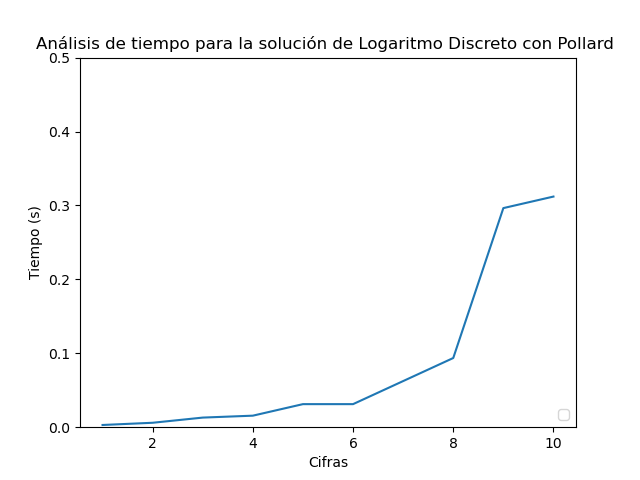
\includegraphics[width=\linewidth]{Figure_9}
        \caption{Análisis de los tiempos de Pollard para PLD.}
        \label{fig:Figure_6}
    \end{figure}
    \newpage
    
    \subsection*{Estimaciones}
    Con el fin de culminar el análisis de tiempos, se realizó una estimación de cuánto tardaría cada algoritmo para encontrar el logaritmo discreto con números de 50 cifras, siguiendo el mismo procedimiento utilizado y descrito en las estimaciones para el problema de Factorización. 
    \newblock
    Por tanto, los resultados encontrados para los algoritmos estudiados en la solución del problema del Logaritmo Discreto son:
    \begin{itemize}
        \item Fuerza Bruta: 6.049137297025345e+40 segundos
        \item Paso Enano - Paso Gigante: 3.2034097360818825e+56 segundos
        \item Ro de Pollard: 6840737595 segundos
    \end{itemize}
    
    \subsection*{Conclusiones de análisis de tiempos para logaritmo Discreto}
    Teniendo en cuenta los datos obtenidos de los tiempos que tarda cada algoritmo en encontrar la solución del logaritmo con determinada cantidad de cifras y la estimación realizada del tiempo en el que se resuelve el logaritmo con números de 50 cifras, evidenciamos que el algoritmo Ro de Pollard es el que mejor comportamiento presenta ya que es el que menos tiempo tarda en resolver el problema. Ejemplo de ello es que para resolver logaritmos con 10 cifras tarda alrededor de 0.4 segundos en comparación a los 191 segundos que gasta el algoritmo Paso Enano - Paso Gigante y la incapacidad de llegar a la solución con este número de cifras con el algoritmo Fuerza Bruta.
    \newblock
    De igual forma, Ro de Pollard resulta eficiente respecto a la estimación de tiempo con 50 cifras dado que demoraría alrededor de 216.91 años para llegar a la solución, cantidad mucho menor a los billones de años que demorarían los algoritmos restantes.
    \newblock
    Se indica así que Ro de Pollard es muy superior a Paso Enano - Paso Gigante y Fuerza Bruta, y así mismo se evidencia que el algoritmo menos eficiente es Fuerza Bruta.
    \newblock
    No obstante, los tres algoritmos son exponenciales en el número de cifras.

\end{document}
